\chapter{Introduction}

The Standard Model (SM) of particle physics has been phenomenally successful in describing most of the observed fundamental particles and their interactions. Its predictive powers have been made evidently manifest with the discovery of the Higgs boson in 2012 at the Large Hadron Collider (LHC) at CERN \cite{collaborationObservationNewBoson2012}, as well as with the discovery of the top quark at the Tevatron at Fermilab in 1995 \cite{abachiObservationTopQuark1995}. In fact, eight of the fundamental particles that make up the SM were predicted to exist before their eventual discovery. However, despite its success, there is clear evidence that it does not constitute a complete theory \cite{saikumarExploringFrontiersChallenges2024,garrettDarkMatterPrimer2011} for multiple reasons, including matter-antimatter asymmetry, the neutrino's nonzero mass, the hierarchy problem, the fine-tuning problem of the Higgs, and the inability of this framework to describe gravity. However, this work will focus on a particularly compelling sign of this theory's incompleteness: the existence and abundance of dark matter.

Dark matter (DM) is a form of nonbaryonic matter that does not interact through any of the forces described by the SM (i.e., the electromagnetic, weak, and strong forces) such that its presence was only initially inferred through its gravitational influence. The first signs of its existence can be traced back to J.H. Oort's observations in 1940 which suggested that the velocity distribution of stars in the Milky Way is such that stars should be moving fast enough to escape the gravitational grasp of the observable mass \cite{oortProblemsConcerningStructure1940}. He postulated that a possible explanation (beyond error) is that there is a significant amount of non-luminous matter deepening the gravitational well of the galaxy, holding these stars in their orbits. Later studies by V. Rubin in the 1980s of the rotation curves of 60 spiral galaxies showed that the extent of the galaxy's mass was much larger than what could be attributed to the visible matter \cite{rubinDarkMatterSpiral1983}.

% The evidence for dark matter is not limited to the rotation curves of galaxies. The relatively small scale of the anisotropies observed in the Cosmic Microwave Background (CMB) by COBE (COsmic Background Explorer) are too small to have been the seeds of the formation of large-scale structures in the universe. There must have been charge-neutral matter that was able to start the structural formation before recombination occurred in the early universe. Additionally, precision studies of the CMB fluctuations carried out using WMAP (Wilkinson Microwave Anisotropy Probe) have indicated that the total matter density of the universe is $\Omega_{m}h^2 = 0.1334$, and that only a small fraction of this, $\Omega_{b}h^2 = 0.02260$, is attributable to baryonic matter. The rest, $\Omega_{dm}h^2 = 0.1123$ or about $83\%$ of the total mass density, comes from elusive dark matter. Thus, a substantial amount of the universe's content is nonbaryonic and not described by the SM.

% Numerous models have been proposed to extend the SM to accommodate DM. Among them are supersymmetry and WIMPs, but no signs of these have been observed. Another class of models of particular interest in this work are those that propose that dark matter is composed of stable dark baryons in a confining Hidden Valley sector that interacts with the SM only through a mediator. If we assume the cogeneration of dark matter and baryonic matter in the early universe through the same mechanism, then we could simultaneously explain the matter-antimatter asymmetry, the dark matter abundance, and the coincidence of mass and number density of DM and baryonic matter. Moreover, this class of models would be consistent with astronomical observations indicating that dark matter is cold and has large self-interactions.

Since the time of Oort and Rubin's evidence has been mounting in favor of the existence of this illusory type of matter. Alongside this evidence, there have been a multitude of proposed models\footnote{Description of this evidence, as well as some of the proposed models, can be found in Section \ref{sec:DM}.}. In this work, we consider a class of DM models that propose that it is composed of stable dark baryons in a confining Hidden Valley sector that interacts with the SM only through a mediator. If we assume the cogeneration of dark matter and baryonic matter in the early universe through the same mechanism, then we could simultaneously explain the matter-antimatter asymmetry, the dark matter abundance, and the coincidence of mass and number density of DM and baryonic matter\cite{schwallerEmergingJets2015}. Moreover, this class of models would be consistent with astronomical observations indicating that dark matter is cold and has large self-interactions.

More particularly, we consider DS models with a TeV-scale mediator. For this class of models, when the dark quarks are produced, their energies will be higher than the confinement scale $\Lambda_D$ of the dark gauge group, resulting in the hadronization of dark quarks into dark hadrons \cite{schwallerEmergingJets2015, albouyTheoryPhenomenologyExperimental2022}. Assuming the dark sector is QCD-like, this process will produce dark jets. Some of the dark hadrons forming part of these jets could be unstable and decay back into SM particles through the mediator. If we consider the lifetime of these unstable particles to be long, they would travel a potentially macroscopic distance before decaying, producing a detectable particle shower. However, because this decay would be a stochastic process, the energy from the dark jet would \textit{emerge} into our detector as the dark hadrons decay back into detectable SM particles. This emerging jet (EMJ) would have to be wide and have a displaced vertex, and its detection would serve as a smoking gun for composite dark-sector models\cite{schwallerEmergingJets2015}. Figure \ref{fig:emj} shows a schematic representation of what such objects might look like in a detector.

% TODO: MAKE MY OWN GRAPHIC AND INCLUDE HERE
\begin{figure}[ht]
	\centering
	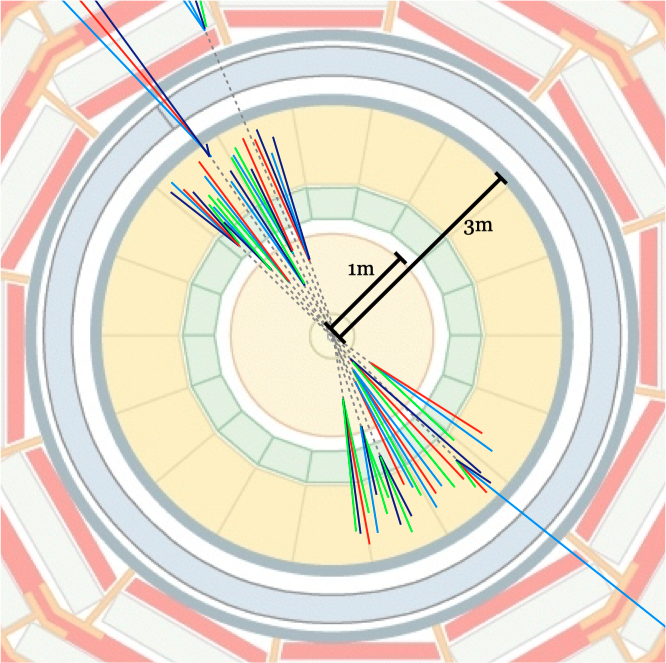
\includegraphics[width=0.5\textwidth]{images/emj.png}
	\caption{Schematic depiction of two EMJs produced through the pair production of dark quarks. The dark quarks hadronize into dark hadrons, some of which are unstable and decay back into SM particles after some distance. The energy from these decays emerges into the detector, producing a wide jet with a displaced vertex \cite{schwallerEmergingJets2015}}.
	\label{fig:emj}
\end{figure}

% EMJs at the LHC
Previous searches for EMJs at the Large Hadron Collider have focused on models with dark-meson lifetimes inside the tracker volume of the CMS detector\cite{}. Moreover, since there was no dedicated EMJ trigger, these searches used triggers that cut on the scalar sum of transverse momenta of jets, or $H_T$. Events with high jet activity would be selected, particularly for the models considered in these searches, which focused on the pair production of bifundamental scalar mediators leading to the production of two EMJs and two QCD jets.

The next phase of the analysis looks towards the inclusion of models in which the mediator is a neutral vector boson, which leads to the production of just two EMJs. This new model leads to signals that are more difficult to find, as the EMJs are softer and the multi-jet QCD background would dominate. In addition to a new mediator, the new search looks to include models with longer-lived dark pions, such that they would mostly decay outside of the tracker volume.

With these new domains in sight for the Run 3 phase of the analysis, a new trigger strategy is needed to ensure adequate sensitivity. In this work, we present trigger efficiency studies performed for a set of novel triggers, namely machine learning (ML) based anomaly detection (AD) triggers and long-lived particle (LLP) triggers, which are implemented in the level-1 (L1) trigger system in CMS.

In order for the EMJ analysis to be conducted, data of the highest quality need to be used, with a guarantee that there are no significant detector issues that have impacted the validity of the physics of the data used. In CMS, a data quality monitoring (DQM) and detector health monitoring infrastructure has been developed since Run 1 that seeks to ensure continuous optimal performance of the detector, as well as reliable data for the analyses performed by the collaboration \cite{DataQualityMonitoring2015, azzoliniDataQualityMonitoring2019}. In order to do this, DQM data are evaluated by experts through careful observation of summary plots that describe detector conditions integrated over an entire run, where a run is a continuous period of data-taking with particular detector conditions that can last minutes to hours.

Although this approach to detector monitoring has proven effective, it requires a considerable amount of person-power, and even all of that work only allows for a per-run evaluation of data, limiting certification granularity. For these reasons, work is underway to integrate ML into the DQM workflow, allowing partial automation of data certification and detector monitoring and increased granularity \cite{wachirapusitanMachineLearningApplications2023, brinkerhoffAnomalyDetectionAutomated2025, CMS-DP-2021-034}. However, particularly for condition-sensitive subdetectors such as the Tracker system, models would need to be frequently retrained, which would require an automated way of selecting reference runs that can serve as training data. In this work, we show a data-driven algorithm dubbed Reference Run Ranking (RRR) developed to offer a curated selection of reference data to use for ML training. In addition, we present data exploration tools developed to enable the granular evaluation of data flagged by models as anomalous. 

In Chapter \ref{chap:SM&beyond} of this work, we will review the Standard Model of particle physics and the specifics of the dark sector models under consideration. In Chapter \ref{chap:CMS}, an overview of the CMS detector will be provided, including a description of each subsystem, and on the trigger system and DQM infrastructure. In Chapter \ref{chap:eventgen}, a discussion of the event generation for the samples used in these studies is discussed. In Chapter \ref{chap:trigeff}, we present the results of the trigger efficiency studies for the novel triggers, followed by a discussion of the RRR algorithm and data exploration tools in Chapter \ref{chap:trackdqm}. Finally, in Chapter \ref{chap:conclusions}, we present the prospects for the Run 3 phase of the EMJ analysis and the future of the search for EMJs at the LHC, as well as the integration of ML to the DQM workflow.